% Created by tikzDevice version 0.6.2 on 2012-04-24 08:02:18
% !TEX encoding = UTF-8 Unicode
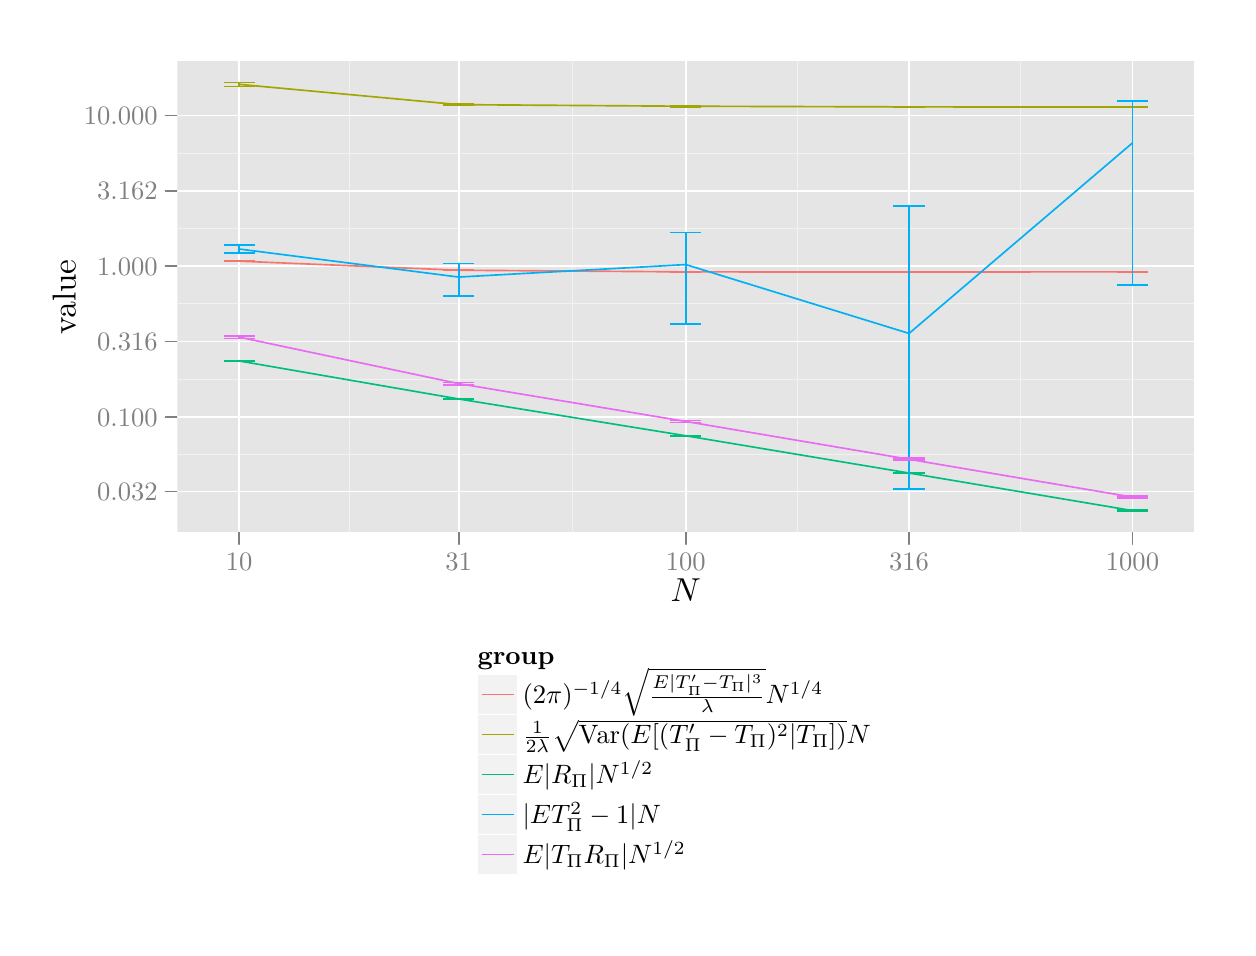
\begin{tikzpicture}[x=1pt,y=1pt]
\definecolor[named]{drawColor}{rgb}{0.00,0.00,0.00}
\definecolor[named]{fillColor}{rgb}{1.00,1.00,1.00}
\fill[color=fillColor,fill opacity=0.00,] (0,0) rectangle (433.62,325.21);
\begin{scope}
\path[clip] (  0.00,  0.00) rectangle (433.62,325.21);
\definecolor[named]{drawColor}{rgb}{0.41,0.16,0.58}
\end{scope}
\begin{scope}
\path[clip] (  0.00,  0.00) rectangle (433.62,325.21);
\definecolor[named]{drawColor}{rgb}{0.41,0.16,0.58}
\end{scope}
\begin{scope}
\path[clip] (  0.00,  0.00) rectangle (433.62,325.21);
\definecolor[named]{drawColor}{rgb}{0.41,0.16,0.58}
\end{scope}
\begin{scope}
\path[clip] (  0.00,  0.00) rectangle (433.62,325.21);
\definecolor[named]{drawColor}{rgb}{0.41,0.16,0.58}
\end{scope}
\begin{scope}
\path[clip] (  0.00,  0.00) rectangle (433.62,325.21);
\definecolor[named]{drawColor}{rgb}{0.41,0.16,0.58}
\end{scope}
\begin{scope}
\path[clip] (  0.00,  0.00) rectangle (433.62,325.21);
\definecolor[named]{drawColor}{rgb}{0.41,0.16,0.58}
\end{scope}
\begin{scope}
\path[clip] (  0.00,  0.00) rectangle (433.62,325.21);
\definecolor[named]{drawColor}{rgb}{0.41,0.16,0.58}
\end{scope}
\begin{scope}
\path[clip] (  0.00,  0.00) rectangle (433.62,325.21);
\definecolor[named]{drawColor}{rgb}{0.41,0.16,0.58}
\end{scope}
\begin{scope}
\path[clip] (  0.00,  0.00) rectangle (433.62,325.21);
\definecolor[named]{drawColor}{rgb}{0.41,0.16,0.58}
\end{scope}
\begin{scope}
\path[clip] (  0.00,  0.00) rectangle (433.62,325.21);
\definecolor[named]{drawColor}{rgb}{0.41,0.16,0.58}
\end{scope}
\begin{scope}
\path[clip] (  0.00,  0.00) rectangle (433.62,325.21);
\definecolor[named]{drawColor}{rgb}{0.41,0.16,0.58}
\end{scope}
\begin{scope}
\path[clip] (  0.00,  0.00) rectangle (433.62,325.21);
\definecolor[named]{drawColor}{rgb}{0.41,0.16,0.58}
\end{scope}
\begin{scope}
\path[clip] ( 54.08,142.81) rectangle (421.57,313.17);
\definecolor[named]{drawColor}{rgb}{0.41,0.16,0.58}
\end{scope}
\begin{scope}
\path[clip] (  0.00,  0.00) rectangle (433.62,325.21);
\definecolor[named]{drawColor}{rgb}{0.41,0.16,0.58}
\end{scope}
\begin{scope}
\path[clip] (  0.00,  0.00) rectangle (433.62,325.21);
\definecolor[named]{drawColor}{rgb}{0.41,0.16,0.58}
\end{scope}
\begin{scope}
\path[clip] (  0.00,  0.00) rectangle (433.62,325.21);
\definecolor[named]{drawColor}{rgb}{0.41,0.16,0.58}
\end{scope}
\begin{scope}
\path[clip] (  0.00,  0.00) rectangle (433.62,325.21);
\definecolor[named]{drawColor}{rgb}{0.41,0.16,0.58}
\end{scope}
\begin{scope}
\path[clip] (  0.00,  0.00) rectangle (433.62,325.21);
\definecolor[named]{drawColor}{rgb}{0.41,0.16,0.58}
\end{scope}
\begin{scope}
\path[clip] (  0.00,  0.00) rectangle (433.62,325.21);
\definecolor[named]{drawColor}{rgb}{0.41,0.16,0.58}
\end{scope}
\begin{scope}
\path[clip] (  0.00,  0.00) rectangle (433.62,325.21);
\definecolor[named]{drawColor}{rgb}{0.41,0.16,0.58}
\end{scope}
\begin{scope}
\path[clip] (  0.00,  0.00) rectangle (433.62,325.21);
\definecolor[named]{drawColor}{rgb}{0.41,0.16,0.58}
\end{scope}
\begin{scope}
\path[clip] (  0.00,  0.00) rectangle (433.62,325.21);
\definecolor[named]{drawColor}{rgb}{0.41,0.16,0.58}
\end{scope}
\begin{scope}
\path[clip] (  0.00,  0.00) rectangle (433.62,325.21);
\definecolor[named]{drawColor}{rgb}{0.41,0.16,0.58}
\end{scope}
\begin{scope}
\path[clip] (  0.00,  0.00) rectangle (433.62,325.21);
\definecolor[named]{drawColor}{rgb}{0.41,0.16,0.58}
\end{scope}
\begin{scope}
\path[clip] (  0.00,  0.00) rectangle (433.62,325.21);
\definecolor[named]{drawColor}{rgb}{0.41,0.16,0.58}
\definecolor[named]{fillColor}{rgb}{1.00,1.00,1.00}

\draw[fill=fillColor,draw opacity=0.00,] (  0.00,  0.00) rectangle (433.62,325.21);
\end{scope}
\begin{scope}
\path[clip] (  0.00,  0.00) rectangle (433.62,325.21);
\definecolor[named]{drawColor}{rgb}{0.41,0.16,0.58}
\end{scope}
\begin{scope}
\path[clip] (  0.00,  0.00) rectangle (433.62,325.21);
\definecolor[named]{drawColor}{rgb}{0.41,0.16,0.58}
\definecolor[named]{drawColor}{rgb}{0.50,0.50,0.50}

\node[color=drawColor,anchor=base east,inner sep=0pt, outer sep=0pt, scale=  0.96] at ( 46.97,154.31) {0.032};

\node[color=drawColor,anchor=base east,inner sep=0pt, outer sep=0pt, scale=  0.96] at ( 46.97,181.26) {0.100};

\node[color=drawColor,anchor=base east,inner sep=0pt, outer sep=0pt, scale=  0.96] at ( 46.97,208.47) {0.316};

\node[color=drawColor,anchor=base east,inner sep=0pt, outer sep=0pt, scale=  0.96] at ( 46.97,235.72) {1.000};

\node[color=drawColor,anchor=base east,inner sep=0pt, outer sep=0pt, scale=  0.96] at ( 46.97,262.94) {3.162};

\node[color=drawColor,anchor=base east,inner sep=0pt, outer sep=0pt, scale=  0.96] at ( 46.97,290.17) {10.000};
\end{scope}
\begin{scope}
\path[clip] (  0.00,  0.00) rectangle (433.62,325.21);
\definecolor[named]{drawColor}{rgb}{0.41,0.16,0.58}
\definecolor[named]{drawColor}{rgb}{0.50,0.50,0.50}

\draw[color=drawColor,line width= 0.6pt,line cap=round,line join=round,fill opacity=0.00,] ( 49.82,157.62) -- ( 54.08,157.62);

\draw[color=drawColor,line width= 0.6pt,line cap=round,line join=round,fill opacity=0.00,] ( 49.82,184.56) -- ( 54.08,184.56);

\draw[color=drawColor,line width= 0.6pt,line cap=round,line join=round,fill opacity=0.00,] ( 49.82,211.78) -- ( 54.08,211.78);

\draw[color=drawColor,line width= 0.6pt,line cap=round,line join=round,fill opacity=0.00,] ( 49.82,239.02) -- ( 54.08,239.02);

\draw[color=drawColor,line width= 0.6pt,line cap=round,line join=round,fill opacity=0.00,] ( 49.82,266.25) -- ( 54.08,266.25);

\draw[color=drawColor,line width= 0.6pt,line cap=round,line join=round,fill opacity=0.00,] ( 49.82,293.48) -- ( 54.08,293.48);
\end{scope}
\begin{scope}
\path[clip] (  0.00,  0.00) rectangle (433.62,325.21);
\definecolor[named]{drawColor}{rgb}{0.41,0.16,0.58}
\end{scope}
\begin{scope}
\path[clip] (  0.00,  0.00) rectangle (433.62,325.21);
\definecolor[named]{drawColor}{rgb}{0.41,0.16,0.58}
\end{scope}
\begin{scope}
\path[clip] (  0.00,  0.00) rectangle (433.62,325.21);
\definecolor[named]{drawColor}{rgb}{0.41,0.16,0.58}
\end{scope}
\begin{scope}
\path[clip] (  0.00,  0.00) rectangle (433.62,325.21);
\definecolor[named]{drawColor}{rgb}{0.41,0.16,0.58}
\end{scope}
\begin{scope}
\path[clip] (  0.00,  0.00) rectangle (433.62,325.21);
\definecolor[named]{drawColor}{rgb}{0.41,0.16,0.58}
\end{scope}
\begin{scope}
\path[clip] ( 54.08,142.81) rectangle (421.57,313.17);
\definecolor[named]{drawColor}{rgb}{0.41,0.16,0.58}
\definecolor[named]{fillColor}{rgb}{0.90,0.90,0.90}

\draw[fill=fillColor,draw opacity=0.00,] ( 54.08,142.81) rectangle (421.57,313.17);
\definecolor[named]{drawColor}{rgb}{0.95,0.95,0.95}

\draw[color=drawColor,line width= 0.3pt,line cap=round,line join=round,fill opacity=0.00,] ( 54.08,171.09) --
	(421.57,171.09);

\draw[color=drawColor,line width= 0.3pt,line cap=round,line join=round,fill opacity=0.00,] ( 54.08,198.17) --
	(421.57,198.17);

\draw[color=drawColor,line width= 0.3pt,line cap=round,line join=round,fill opacity=0.00,] ( 54.08,225.40) --
	(421.57,225.40);

\draw[color=drawColor,line width= 0.3pt,line cap=round,line join=round,fill opacity=0.00,] ( 54.08,252.64) --
	(421.57,252.64);

\draw[color=drawColor,line width= 0.3pt,line cap=round,line join=round,fill opacity=0.00,] ( 54.08,279.87) --
	(421.57,279.87);

\draw[color=drawColor,line width= 0.3pt,line cap=round,line join=round,fill opacity=0.00,] (116.09,142.81) --
	(116.09,313.17);

\draw[color=drawColor,line width= 0.3pt,line cap=round,line join=round,fill opacity=0.00,] (196.78,142.81) --
	(196.78,313.17);

\draw[color=drawColor,line width= 0.3pt,line cap=round,line join=round,fill opacity=0.00,] (278.15,142.81) --
	(278.15,313.17);

\draw[color=drawColor,line width= 0.3pt,line cap=round,line join=round,fill opacity=0.00,] (358.85,142.81) --
	(358.85,313.17);
\definecolor[named]{drawColor}{rgb}{1.00,1.00,1.00}

\draw[color=drawColor,line width= 0.6pt,line cap=round,line join=round,fill opacity=0.00,] ( 54.08,157.62) --
	(421.57,157.62);

\draw[color=drawColor,line width= 0.6pt,line cap=round,line join=round,fill opacity=0.00,] ( 54.08,184.56) --
	(421.57,184.56);

\draw[color=drawColor,line width= 0.6pt,line cap=round,line join=round,fill opacity=0.00,] ( 54.08,211.78) --
	(421.57,211.78);

\draw[color=drawColor,line width= 0.6pt,line cap=round,line join=round,fill opacity=0.00,] ( 54.08,239.02) --
	(421.57,239.02);

\draw[color=drawColor,line width= 0.6pt,line cap=round,line join=round,fill opacity=0.00,] ( 54.08,266.25) --
	(421.57,266.25);

\draw[color=drawColor,line width= 0.6pt,line cap=round,line join=round,fill opacity=0.00,] ( 54.08,293.48) --
	(421.57,293.48);

\draw[color=drawColor,line width= 0.6pt,line cap=round,line join=round,fill opacity=0.00,] ( 76.44,142.81) --
	( 76.44,313.17);

\draw[color=drawColor,line width= 0.6pt,line cap=round,line join=round,fill opacity=0.00,] (155.74,142.81) --
	(155.74,313.17);

\draw[color=drawColor,line width= 0.6pt,line cap=round,line join=round,fill opacity=0.00,] (237.83,142.81) --
	(237.83,313.17);

\draw[color=drawColor,line width= 0.6pt,line cap=round,line join=round,fill opacity=0.00,] (318.48,142.81) --
	(318.48,313.17);

\draw[color=drawColor,line width= 0.6pt,line cap=round,line join=round,fill opacity=0.00,] (399.22,142.81) --
	(399.22,313.17);
\definecolor[named]{drawColor}{rgb}{0.97,0.46,0.43}

\draw[color=drawColor,line width= 0.6pt,line join=round,fill opacity=0.00,] ( 76.44,240.84) --
	(155.74,237.56) --
	(237.83,236.96) --
	(318.48,236.91) --
	(399.22,236.98);
\definecolor[named]{drawColor}{rgb}{0.64,0.65,0.00}

\draw[color=drawColor,line width= 0.6pt,line join=round,fill opacity=0.00,] ( 76.44,304.72) --
	(155.74,297.39) --
	(237.83,296.82) --
	(318.48,296.58) --
	(399.22,296.53);
\definecolor[named]{drawColor}{rgb}{0.00,0.75,0.49}

\draw[color=drawColor,line width= 0.6pt,line join=round,fill opacity=0.00,] ( 76.44,204.77) --
	(155.74,191.04) --
	(237.83,177.74) --
	(318.48,164.27) --
	(399.22,150.70);
\definecolor[named]{drawColor}{rgb}{0.00,0.69,0.96}

\draw[color=drawColor,line width= 0.6pt,line join=round,fill opacity=0.00,] ( 76.44,245.22) --
	(155.74,235.09) --
	(237.83,239.60) --
	(318.48,214.72) --
	(399.22,283.56);
\definecolor[named]{drawColor}{rgb}{0.91,0.42,0.95}

\draw[color=drawColor,line width= 0.6pt,line join=round,fill opacity=0.00,] ( 76.44,213.38) --
	(155.74,196.58) --
	(237.83,182.91) --
	(318.48,169.24) --
	(399.22,155.57);
\definecolor[named]{drawColor}{rgb}{0.97,0.46,0.43}

\draw[color=drawColor,line width= 0.6pt,line join=round,fill opacity=0.00,] ( 70.79,240.89) --
	( 82.08,240.89);

\draw[color=drawColor,line width= 0.6pt,line join=round,fill opacity=0.00,] ( 76.44,240.89) --
	( 76.44,240.78);

\draw[color=drawColor,line width= 0.6pt,line join=round,fill opacity=0.00,] ( 70.79,240.78) --
	( 82.08,240.78);

\draw[color=drawColor,line width= 0.6pt,line join=round,fill opacity=0.00,] (150.09,237.57) --
	(161.39,237.57);

\draw[color=drawColor,line width= 0.6pt,line join=round,fill opacity=0.00,] (155.74,237.57) --
	(155.74,237.56);

\draw[color=drawColor,line width= 0.6pt,line join=round,fill opacity=0.00,] (150.09,237.56) --
	(161.39,237.56);

\draw[color=drawColor,line width= 0.6pt,line join=round,fill opacity=0.00,] (232.18,236.96) --
	(243.48,236.96);

\draw[color=drawColor,line width= 0.6pt,line join=round,fill opacity=0.00,] (237.83,236.96) --
	(237.83,236.96);

\draw[color=drawColor,line width= 0.6pt,line join=round,fill opacity=0.00,] (232.18,236.96) --
	(243.48,236.96);

\draw[color=drawColor,line width= 0.6pt,line join=round,fill opacity=0.00,] (312.83,236.91) --
	(324.12,236.91);

\draw[color=drawColor,line width= 0.6pt,line join=round,fill opacity=0.00,] (318.48,236.91) --
	(318.48,236.91);

\draw[color=drawColor,line width= 0.6pt,line join=round,fill opacity=0.00,] (312.83,236.91) --
	(324.12,236.91);

\draw[color=drawColor,line width= 0.6pt,line join=round,fill opacity=0.00,] (393.57,236.98) --
	(404.87,236.98);

\draw[color=drawColor,line width= 0.6pt,line join=round,fill opacity=0.00,] (399.22,236.98) --
	(399.22,236.98);

\draw[color=drawColor,line width= 0.6pt,line join=round,fill opacity=0.00,] (393.57,236.98) --
	(404.87,236.98);
\definecolor[named]{drawColor}{rgb}{0.64,0.65,0.00}

\draw[color=drawColor,line width= 0.6pt,line join=round,fill opacity=0.00,] ( 70.79,305.43) --
	( 82.08,305.43);

\draw[color=drawColor,line width= 0.6pt,line join=round,fill opacity=0.00,] ( 76.44,305.43) --
	( 76.44,304.01);

\draw[color=drawColor,line width= 0.6pt,line join=round,fill opacity=0.00,] ( 70.79,304.01) --
	( 82.08,304.01);

\draw[color=drawColor,line width= 0.6pt,line join=round,fill opacity=0.00,] (150.09,297.68) --
	(161.39,297.68);

\draw[color=drawColor,line width= 0.6pt,line join=round,fill opacity=0.00,] (155.74,297.68) --
	(155.74,297.13);

\draw[color=drawColor,line width= 0.6pt,line join=round,fill opacity=0.00,] (150.09,297.13) --
	(161.39,297.13);

\draw[color=drawColor,line width= 0.6pt,line join=round,fill opacity=0.00,] (232.18,297.05) --
	(243.48,297.05);

\draw[color=drawColor,line width= 0.6pt,line join=round,fill opacity=0.00,] (237.83,297.05) --
	(237.83,296.59);

\draw[color=drawColor,line width= 0.6pt,line join=round,fill opacity=0.00,] (232.18,296.59) --
	(243.48,296.59);

\draw[color=drawColor,line width= 0.6pt,line join=round,fill opacity=0.00,] (312.83,296.77) --
	(324.12,296.77);

\draw[color=drawColor,line width= 0.6pt,line join=round,fill opacity=0.00,] (318.48,296.77) --
	(318.48,296.39);

\draw[color=drawColor,line width= 0.6pt,line join=round,fill opacity=0.00,] (312.83,296.39) --
	(324.12,296.39);

\draw[color=drawColor,line width= 0.6pt,line join=round,fill opacity=0.00,] (393.57,296.72) --
	(404.87,296.72);

\draw[color=drawColor,line width= 0.6pt,line join=round,fill opacity=0.00,] (399.22,296.72) --
	(399.22,296.35);

\draw[color=drawColor,line width= 0.6pt,line join=round,fill opacity=0.00,] (393.57,296.35) --
	(404.87,296.35);
\definecolor[named]{drawColor}{rgb}{0.00,0.75,0.49}

\draw[color=drawColor,line width= 0.6pt,line join=round,fill opacity=0.00,] ( 70.79,204.94) --
	( 82.08,204.94);

\draw[color=drawColor,line width= 0.6pt,line join=round,fill opacity=0.00,] ( 76.44,204.94) --
	( 76.44,204.60);

\draw[color=drawColor,line width= 0.6pt,line join=round,fill opacity=0.00,] ( 70.79,204.60) --
	( 82.08,204.60);

\draw[color=drawColor,line width= 0.6pt,line join=round,fill opacity=0.00,] (150.09,191.19) --
	(161.39,191.19);

\draw[color=drawColor,line width= 0.6pt,line join=round,fill opacity=0.00,] (155.74,191.19) --
	(155.74,190.91);

\draw[color=drawColor,line width= 0.6pt,line join=round,fill opacity=0.00,] (150.09,190.91) --
	(161.39,190.91);

\draw[color=drawColor,line width= 0.6pt,line join=round,fill opacity=0.00,] (232.18,177.87) --
	(243.48,177.87);

\draw[color=drawColor,line width= 0.6pt,line join=round,fill opacity=0.00,] (237.83,177.87) --
	(237.83,177.59);

\draw[color=drawColor,line width= 0.6pt,line join=round,fill opacity=0.00,] (232.18,177.59) --
	(243.48,177.59);

\draw[color=drawColor,line width= 0.6pt,line join=round,fill opacity=0.00,] (312.83,164.39) --
	(324.12,164.39);

\draw[color=drawColor,line width= 0.6pt,line join=round,fill opacity=0.00,] (318.48,164.39) --
	(318.48,164.14);

\draw[color=drawColor,line width= 0.6pt,line join=round,fill opacity=0.00,] (312.83,164.14) --
	(324.12,164.14);

\draw[color=drawColor,line width= 0.6pt,line join=round,fill opacity=0.00,] (393.57,150.82) --
	(404.87,150.82);

\draw[color=drawColor,line width= 0.6pt,line join=round,fill opacity=0.00,] (399.22,150.82) --
	(399.22,150.56);

\draw[color=drawColor,line width= 0.6pt,line join=round,fill opacity=0.00,] (393.57,150.56) --
	(404.87,150.56);
\definecolor[named]{drawColor}{rgb}{0.00,0.69,0.96}

\draw[color=drawColor,line width= 0.6pt,line join=round,fill opacity=0.00,] ( 70.79,246.60) --
	( 82.08,246.60);

\draw[color=drawColor,line width= 0.6pt,line join=round,fill opacity=0.00,] ( 76.44,246.60) --
	( 76.44,243.72);

\draw[color=drawColor,line width= 0.6pt,line join=round,fill opacity=0.00,] ( 70.79,243.72) --
	( 82.08,243.72);

\draw[color=drawColor,line width= 0.6pt,line join=round,fill opacity=0.00,] (150.09,239.93) --
	(161.39,239.93);

\draw[color=drawColor,line width= 0.6pt,line join=round,fill opacity=0.00,] (155.74,239.93) --
	(155.74,228.31);

\draw[color=drawColor,line width= 0.6pt,line join=round,fill opacity=0.00,] (150.09,228.31) --
	(161.39,228.31);

\draw[color=drawColor,line width= 0.6pt,line join=round,fill opacity=0.00,] (232.18,251.16) --
	(243.48,251.16);

\draw[color=drawColor,line width= 0.6pt,line join=round,fill opacity=0.00,] (237.83,251.16) --
	(237.83,218.23);

\draw[color=drawColor,line width= 0.6pt,line join=round,fill opacity=0.00,] (232.18,218.23) --
	(243.48,218.23);

\draw[color=drawColor,line width= 0.6pt,line join=round,fill opacity=0.00,] (312.83,260.65) --
	(324.12,260.65);

\draw[color=drawColor,line width= 0.6pt,line join=round,fill opacity=0.00,] (318.48,260.65) --
	(318.48,158.40);

\draw[color=drawColor,line width= 0.6pt,line join=round,fill opacity=0.00,] (312.83,158.40) --
	(324.12,158.40);

\draw[color=drawColor,line width= 0.6pt,line join=round,fill opacity=0.00,] (393.57,298.71) --
	(404.87,298.71);

\draw[color=drawColor,line width= 0.6pt,line join=round,fill opacity=0.00,] (399.22,298.71) --
	(399.22,232.33);

\draw[color=drawColor,line width= 0.6pt,line join=round,fill opacity=0.00,] (393.57,232.33) --
	(404.87,232.33);
\definecolor[named]{drawColor}{rgb}{0.91,0.42,0.95}

\draw[color=drawColor,line width= 0.6pt,line join=round,fill opacity=0.00,] ( 70.79,213.89) --
	( 82.08,213.89);

\draw[color=drawColor,line width= 0.6pt,line join=round,fill opacity=0.00,] ( 76.44,213.89) --
	( 76.44,212.86);

\draw[color=drawColor,line width= 0.6pt,line join=round,fill opacity=0.00,] ( 70.79,212.86) --
	( 82.08,212.86);

\draw[color=drawColor,line width= 0.6pt,line join=round,fill opacity=0.00,] (150.09,196.96) --
	(161.39,196.96);

\draw[color=drawColor,line width= 0.6pt,line join=round,fill opacity=0.00,] (155.74,196.96) --
	(155.74,196.20);

\draw[color=drawColor,line width= 0.6pt,line join=round,fill opacity=0.00,] (150.09,196.20) --
	(161.39,196.20);

\draw[color=drawColor,line width= 0.6pt,line join=round,fill opacity=0.00,] (232.18,183.31) --
	(243.48,183.31);

\draw[color=drawColor,line width= 0.6pt,line join=round,fill opacity=0.00,] (237.83,183.31) --
	(237.83,182.54);

\draw[color=drawColor,line width= 0.6pt,line join=round,fill opacity=0.00,] (232.18,182.54) --
	(243.48,182.54);

\draw[color=drawColor,line width= 0.6pt,line join=round,fill opacity=0.00,] (312.83,169.60) --
	(324.12,169.60);

\draw[color=drawColor,line width= 0.6pt,line join=round,fill opacity=0.00,] (318.48,169.60) --
	(318.48,168.89);

\draw[color=drawColor,line width= 0.6pt,line join=round,fill opacity=0.00,] (312.83,168.89) --
	(324.12,168.89);

\draw[color=drawColor,line width= 0.6pt,line join=round,fill opacity=0.00,] (393.57,155.90) --
	(404.87,155.90);

\draw[color=drawColor,line width= 0.6pt,line join=round,fill opacity=0.00,] (399.22,155.90) --
	(399.22,155.26);

\draw[color=drawColor,line width= 0.6pt,line join=round,fill opacity=0.00,] (393.57,155.26) --
	(404.87,155.26);
\end{scope}
\begin{scope}
\path[clip] (  0.00,  0.00) rectangle (433.62,325.21);
\definecolor[named]{drawColor}{rgb}{0.41,0.16,0.58}
\end{scope}
\begin{scope}
\path[clip] (  0.00,  0.00) rectangle (433.62,325.21);
\definecolor[named]{drawColor}{rgb}{0.41,0.16,0.58}
\definecolor[named]{drawColor}{rgb}{0.50,0.50,0.50}

\node[color=drawColor,anchor=base,inner sep=0pt, outer sep=0pt, scale=  0.96] at ( 76.44,129.09) {10};

\node[color=drawColor,anchor=base,inner sep=0pt, outer sep=0pt, scale=  0.96] at (155.74,129.09) {31};

\node[color=drawColor,anchor=base,inner sep=0pt, outer sep=0pt, scale=  0.96] at (237.83,129.09) {100};

\node[color=drawColor,anchor=base,inner sep=0pt, outer sep=0pt, scale=  0.96] at (318.48,129.09) {316};

\node[color=drawColor,anchor=base,inner sep=0pt, outer sep=0pt, scale=  0.96] at (399.22,129.09) {1000};
\end{scope}
\begin{scope}
\path[clip] (  0.00,  0.00) rectangle (433.62,325.21);
\definecolor[named]{drawColor}{rgb}{0.41,0.16,0.58}
\definecolor[named]{drawColor}{rgb}{0.50,0.50,0.50}

\draw[color=drawColor,line width= 0.6pt,line cap=round,line join=round,fill opacity=0.00,] ( 76.44,138.55) -- ( 76.44,142.81);

\draw[color=drawColor,line width= 0.6pt,line cap=round,line join=round,fill opacity=0.00,] (155.74,138.55) -- (155.74,142.81);

\draw[color=drawColor,line width= 0.6pt,line cap=round,line join=round,fill opacity=0.00,] (237.83,138.55) -- (237.83,142.81);

\draw[color=drawColor,line width= 0.6pt,line cap=round,line join=round,fill opacity=0.00,] (318.48,138.55) -- (318.48,142.81);

\draw[color=drawColor,line width= 0.6pt,line cap=round,line join=round,fill opacity=0.00,] (399.22,138.55) -- (399.22,142.81);
\end{scope}
\begin{scope}
\path[clip] (  0.00,  0.00) rectangle (433.62,325.21);
\definecolor[named]{drawColor}{rgb}{0.41,0.16,0.58}
\end{scope}
\begin{scope}
\path[clip] (  0.00,  0.00) rectangle (433.62,325.21);
\definecolor[named]{drawColor}{rgb}{0.41,0.16,0.58}
\end{scope}
\begin{scope}
\path[clip] (  0.00,  0.00) rectangle (433.62,325.21);
\definecolor[named]{drawColor}{rgb}{0.41,0.16,0.58}
\end{scope}
\begin{scope}
\path[clip] (  0.00,  0.00) rectangle (433.62,325.21);
\definecolor[named]{drawColor}{rgb}{0.41,0.16,0.58}
\end{scope}
\begin{scope}
\path[clip] (  0.00,  0.00) rectangle (433.62,325.21);
\definecolor[named]{drawColor}{rgb}{0.41,0.16,0.58}
\end{scope}
\begin{scope}
\path[clip] (  0.00,  0.00) rectangle (433.62,325.21);
\definecolor[named]{drawColor}{rgb}{0.41,0.16,0.58}
\definecolor[named]{drawColor}{rgb}{0.00,0.00,0.00}

\node[color=drawColor,anchor=base,inner sep=0pt, outer sep=0pt, scale=  1.20] at (237.83,117.81) {$N$};
\end{scope}
\begin{scope}
\path[clip] (  0.00,  0.00) rectangle (433.62,325.21);
\definecolor[named]{drawColor}{rgb}{0.41,0.16,0.58}
\end{scope}
\begin{scope}
\path[clip] (  0.00,  0.00) rectangle (433.62,325.21);
\definecolor[named]{drawColor}{rgb}{0.41,0.16,0.58}
\definecolor[named]{drawColor}{rgb}{0.00,0.00,0.00}

\node[rotate= 90.00,color=drawColor,anchor=base,inner sep=0pt, outer sep=0pt, scale=  1.20] at ( 17.30,227.99) {value};
\end{scope}
\begin{scope}
\path[clip] (  0.00,  0.00) rectangle (433.62,325.21);
\definecolor[named]{drawColor}{rgb}{0.41,0.16,0.58}
\end{scope}
\begin{scope}
\path[clip] (  0.00,  0.00) rectangle (433.62,325.21);
\definecolor[named]{drawColor}{rgb}{0.41,0.16,0.58}
\end{scope}
\begin{scope}
\path[clip] (  0.00,  0.00) rectangle (433.62,325.21);
\definecolor[named]{drawColor}{rgb}{0.41,0.16,0.58}
\end{scope}
\begin{scope}
\path[clip] (  0.00,  0.00) rectangle (433.62,325.21);
\definecolor[named]{drawColor}{rgb}{0.41,0.16,0.58}
\end{scope}
\begin{scope}
\path[clip] (  0.00,  0.00) rectangle (433.62,325.21);
\definecolor[named]{drawColor}{rgb}{0.41,0.16,0.58}
\end{scope}
\begin{scope}
\path[clip] (  0.00,  0.00) rectangle (433.62,325.21);
\definecolor[named]{drawColor}{rgb}{0.41,0.16,0.58}
\end{scope}
\begin{scope}
\path[clip] (  0.00,  0.00) rectangle (433.62,325.21);
\definecolor[named]{drawColor}{rgb}{0.41,0.16,0.58}
\end{scope}
\begin{scope}
\path[clip] (  0.00,  0.00) rectangle (433.62,325.21);
\definecolor[named]{drawColor}{rgb}{0.41,0.16,0.58}
\end{scope}
\begin{scope}
\path[clip] (  0.00,  0.00) rectangle (433.62,325.21);
\definecolor[named]{drawColor}{rgb}{0.41,0.16,0.58}
\end{scope}
\begin{scope}
\path[clip] (  0.00,  0.00) rectangle (433.62,325.21);
\definecolor[named]{drawColor}{rgb}{0.41,0.16,0.58}
\end{scope}
\begin{scope}
\path[clip] (  0.00,  0.00) rectangle (433.62,325.21);
\definecolor[named]{drawColor}{rgb}{0.41,0.16,0.58}
\end{scope}
\begin{scope}
\path[clip] (  0.00,  0.00) rectangle (433.62,325.21);
\definecolor[named]{drawColor}{rgb}{0.41,0.16,0.58}
\end{scope}
\begin{scope}
\path[clip] (  0.00,  0.00) rectangle (433.62,325.21);
\definecolor[named]{drawColor}{rgb}{0.41,0.16,0.58}
\end{scope}
\begin{scope}
\path[clip] (  0.00,  0.00) rectangle (433.62,325.21);
\definecolor[named]{drawColor}{rgb}{0.41,0.16,0.58}
\end{scope}
\begin{scope}
\path[clip] (  0.00,  0.00) rectangle (433.62,325.21);
\definecolor[named]{drawColor}{rgb}{0.41,0.16,0.58}
\end{scope}
\begin{scope}
\path[clip] (  0.00,  0.00) rectangle (433.62,325.21);
\definecolor[named]{drawColor}{rgb}{0.41,0.16,0.58}
\end{scope}
\begin{scope}
\path[clip] (  0.00,  0.00) rectangle (433.62,325.21);
\definecolor[named]{drawColor}{rgb}{0.41,0.16,0.58}
\end{scope}
\begin{scope}
\path[clip] (  0.00,  0.00) rectangle (433.62,325.21);
\definecolor[named]{drawColor}{rgb}{0.41,0.16,0.58}
\end{scope}
\begin{scope}
\path[clip] (  0.00,  0.00) rectangle (433.62,325.21);
\definecolor[named]{drawColor}{rgb}{0.41,0.16,0.58}
\end{scope}
\begin{scope}
\path[clip] (  0.00,  0.00) rectangle (433.62,325.21);
\definecolor[named]{drawColor}{rgb}{0.41,0.16,0.58}
\end{scope}
\begin{scope}
\path[clip] (  0.00,  0.00) rectangle (433.62,325.21);
\definecolor[named]{drawColor}{rgb}{0.41,0.16,0.58}
\end{scope}
\begin{scope}
\path[clip] (  0.00,  0.00) rectangle (433.62,325.21);
\definecolor[named]{drawColor}{rgb}{0.41,0.16,0.58}
\end{scope}
\begin{scope}
\path[clip] (  0.00,  0.00) rectangle (433.62,325.21);
\definecolor[named]{drawColor}{rgb}{0.41,0.16,0.58}
\end{scope}
\begin{scope}
\path[clip] (  0.00,  0.00) rectangle (433.62,325.21);
\definecolor[named]{drawColor}{rgb}{0.41,0.16,0.58}
\end{scope}
\begin{scope}
\path[clip] (  0.00,  0.00) rectangle (433.62,325.21);
\definecolor[named]{drawColor}{rgb}{0.41,0.16,0.58}
\definecolor[named]{drawColor}{rgb}{1.00,1.00,1.00}

\draw[color=drawColor,line width= 0.6pt,line cap=round,line join=round,fill opacity=0.00,] (158.31, 14.89) rectangle (317.35,105.93);
\end{scope}
\begin{scope}
\path[clip] (  0.00,  0.00) rectangle (433.62,325.21);
\definecolor[named]{drawColor}{rgb}{0.41,0.16,0.58}
\definecolor[named]{drawColor}{rgb}{0.00,0.00,0.00}

\node[color=drawColor,anchor=base west,inner sep=0pt, outer sep=0pt, scale=  0.96] at (162.58, 95.04) {\bfseries group};
\end{scope}
\begin{scope}
\path[clip] (  0.00,  0.00) rectangle (433.62,325.21);
\definecolor[named]{drawColor}{rgb}{0.41,0.16,0.58}
\definecolor[named]{drawColor}{rgb}{1.00,1.00,1.00}
\definecolor[named]{fillColor}{rgb}{0.95,0.95,0.95}

\draw[color=drawColor,line width= 0.6pt,line cap=round,line join=round,fill=fillColor,] (162.58, 76.97) rectangle (177.03, 91.43);
\end{scope}
\begin{scope}
\path[clip] (  0.00,  0.00) rectangle (433.62,325.21);
\definecolor[named]{drawColor}{rgb}{0.41,0.16,0.58}
\definecolor[named]{drawColor}{rgb}{0.97,0.46,0.43}

\draw[color=drawColor,line width= 0.6pt,line join=round,fill opacity=0.00,] (164.02, 84.20) -- (175.58, 84.20);
\end{scope}
\begin{scope}
\path[clip] (  0.00,  0.00) rectangle (433.62,325.21);
\definecolor[named]{drawColor}{rgb}{0.41,0.16,0.58}
\definecolor[named]{drawColor}{rgb}{0.97,0.46,0.43}

\draw[color=drawColor,line width= 0.6pt,line join=round,fill opacity=0.00,] (164.02, 84.20) -- (175.58, 84.20);
\end{scope}
\begin{scope}
\path[clip] (  0.00,  0.00) rectangle (433.62,325.21);
\definecolor[named]{drawColor}{rgb}{0.41,0.16,0.58}
\definecolor[named]{drawColor}{rgb}{1.00,1.00,1.00}
\definecolor[named]{fillColor}{rgb}{0.95,0.95,0.95}

\draw[color=drawColor,line width= 0.6pt,line cap=round,line join=round,fill=fillColor,] (162.58, 62.52) rectangle (177.03, 76.97);
\end{scope}
\begin{scope}
\path[clip] (  0.00,  0.00) rectangle (433.62,325.21);
\definecolor[named]{drawColor}{rgb}{0.41,0.16,0.58}
\definecolor[named]{drawColor}{rgb}{0.64,0.65,0.00}

\draw[color=drawColor,line width= 0.6pt,line join=round,fill opacity=0.00,] (164.02, 69.75) -- (175.58, 69.75);
\end{scope}
\begin{scope}
\path[clip] (  0.00,  0.00) rectangle (433.62,325.21);
\definecolor[named]{drawColor}{rgb}{0.41,0.16,0.58}
\definecolor[named]{drawColor}{rgb}{0.64,0.65,0.00}

\draw[color=drawColor,line width= 0.6pt,line join=round,fill opacity=0.00,] (164.02, 69.75) -- (175.58, 69.75);
\end{scope}
\begin{scope}
\path[clip] (  0.00,  0.00) rectangle (433.62,325.21);
\definecolor[named]{drawColor}{rgb}{0.41,0.16,0.58}
\definecolor[named]{drawColor}{rgb}{1.00,1.00,1.00}
\definecolor[named]{fillColor}{rgb}{0.95,0.95,0.95}

\draw[color=drawColor,line width= 0.6pt,line cap=round,line join=round,fill=fillColor,] (162.58, 48.07) rectangle (177.03, 62.52);
\end{scope}
\begin{scope}
\path[clip] (  0.00,  0.00) rectangle (433.62,325.21);
\definecolor[named]{drawColor}{rgb}{0.41,0.16,0.58}
\definecolor[named]{drawColor}{rgb}{0.00,0.75,0.49}

\draw[color=drawColor,line width= 0.6pt,line join=round,fill opacity=0.00,] (164.02, 55.29) -- (175.58, 55.29);
\end{scope}
\begin{scope}
\path[clip] (  0.00,  0.00) rectangle (433.62,325.21);
\definecolor[named]{drawColor}{rgb}{0.41,0.16,0.58}
\definecolor[named]{drawColor}{rgb}{0.00,0.75,0.49}

\draw[color=drawColor,line width= 0.6pt,line join=round,fill opacity=0.00,] (164.02, 55.29) -- (175.58, 55.29);
\end{scope}
\begin{scope}
\path[clip] (  0.00,  0.00) rectangle (433.62,325.21);
\definecolor[named]{drawColor}{rgb}{0.41,0.16,0.58}
\definecolor[named]{drawColor}{rgb}{1.00,1.00,1.00}
\definecolor[named]{fillColor}{rgb}{0.95,0.95,0.95}

\draw[color=drawColor,line width= 0.6pt,line cap=round,line join=round,fill=fillColor,] (162.58, 33.61) rectangle (177.03, 48.07);
\end{scope}
\begin{scope}
\path[clip] (  0.00,  0.00) rectangle (433.62,325.21);
\definecolor[named]{drawColor}{rgb}{0.41,0.16,0.58}
\definecolor[named]{drawColor}{rgb}{0.00,0.69,0.96}

\draw[color=drawColor,line width= 0.6pt,line join=round,fill opacity=0.00,] (164.02, 40.84) -- (175.58, 40.84);
\end{scope}
\begin{scope}
\path[clip] (  0.00,  0.00) rectangle (433.62,325.21);
\definecolor[named]{drawColor}{rgb}{0.41,0.16,0.58}
\definecolor[named]{drawColor}{rgb}{0.00,0.69,0.96}

\draw[color=drawColor,line width= 0.6pt,line join=round,fill opacity=0.00,] (164.02, 40.84) -- (175.58, 40.84);
\end{scope}
\begin{scope}
\path[clip] (  0.00,  0.00) rectangle (433.62,325.21);
\definecolor[named]{drawColor}{rgb}{0.41,0.16,0.58}
\definecolor[named]{drawColor}{rgb}{1.00,1.00,1.00}
\definecolor[named]{fillColor}{rgb}{0.95,0.95,0.95}

\draw[color=drawColor,line width= 0.6pt,line cap=round,line join=round,fill=fillColor,] (162.58, 19.16) rectangle (177.03, 33.61);
\end{scope}
\begin{scope}
\path[clip] (  0.00,  0.00) rectangle (433.62,325.21);
\definecolor[named]{drawColor}{rgb}{0.41,0.16,0.58}
\definecolor[named]{drawColor}{rgb}{0.91,0.42,0.95}

\draw[color=drawColor,line width= 0.6pt,line join=round,fill opacity=0.00,] (164.02, 26.39) -- (175.58, 26.39);
\end{scope}
\begin{scope}
\path[clip] (  0.00,  0.00) rectangle (433.62,325.21);
\definecolor[named]{drawColor}{rgb}{0.41,0.16,0.58}
\definecolor[named]{drawColor}{rgb}{0.91,0.42,0.95}

\draw[color=drawColor,line width= 0.6pt,line join=round,fill opacity=0.00,] (164.02, 26.39) -- (175.58, 26.39);
\end{scope}
\begin{scope}
\path[clip] (  0.00,  0.00) rectangle (433.62,325.21);
\definecolor[named]{drawColor}{rgb}{0.41,0.16,0.58}
\definecolor[named]{drawColor}{rgb}{0.00,0.00,0.00}

\node[color=drawColor,anchor=base west,inner sep=0pt, outer sep=0pt, scale=  0.96] at (178.84, 80.90) {$(2\pi)^{-1/4}\sqrt{\frac{\mathbb{E}|T'_{\Pi}-T_{\Pi}|^3}{\lambda}}N^{1/4}\quad $};
\end{scope}
\begin{scope}
\path[clip] (  0.00,  0.00) rectangle (433.62,325.21);
\definecolor[named]{drawColor}{rgb}{0.41,0.16,0.58}
\definecolor[named]{drawColor}{rgb}{0.00,0.00,0.00}

\node[color=drawColor,anchor=base west,inner sep=0pt, outer sep=0pt, scale=  0.96] at (178.84, 66.44) {$\frac{1}{2\lambda}\sqrt{\mathrm{Var}(\mathbb{E}[(T'_{\Pi}-T_{\Pi})^2|T_{\Pi}])}N\quad $};
\end{scope}
\begin{scope}
\path[clip] (  0.00,  0.00) rectangle (433.62,325.21);
\definecolor[named]{drawColor}{rgb}{0.41,0.16,0.58}
\definecolor[named]{drawColor}{rgb}{0.00,0.00,0.00}

\node[color=drawColor,anchor=base west,inner sep=0pt, outer sep=0pt, scale=  0.96] at (178.84, 51.99) {$\mathbb{E}|R_{\Pi}|N^{1/2}\quad $};
\end{scope}
\begin{scope}
\path[clip] (  0.00,  0.00) rectangle (433.62,325.21);
\definecolor[named]{drawColor}{rgb}{0.41,0.16,0.58}
\definecolor[named]{drawColor}{rgb}{0.00,0.00,0.00}

\node[color=drawColor,anchor=base west,inner sep=0pt, outer sep=0pt, scale=  0.96] at (178.84, 37.53) {$|\mathbb{E}T_{\Pi}^2-1|N\quad $};
\end{scope}
\begin{scope}
\path[clip] (  0.00,  0.00) rectangle (433.62,325.21);
\definecolor[named]{drawColor}{rgb}{0.41,0.16,0.58}
\definecolor[named]{drawColor}{rgb}{0.00,0.00,0.00}

\node[color=drawColor,anchor=base west,inner sep=0pt, outer sep=0pt, scale=  0.96] at (178.84, 23.08) {$\mathbb{E}|T_{\Pi}R_{\Pi}|N^{1/2}\quad $};
\end{scope}
\begin{scope}
\path[clip] (  0.00,  0.00) rectangle (433.62,325.21);
\definecolor[named]{drawColor}{rgb}{0.41,0.16,0.58}
\end{scope}
\begin{scope}
\path[clip] (  0.00,  0.00) rectangle (433.62,325.21);
\definecolor[named]{drawColor}{rgb}{0.41,0.16,0.58}
\end{scope}
\begin{scope}
\path[clip] (  0.00,  0.00) rectangle (433.62,325.21);
\definecolor[named]{drawColor}{rgb}{0.41,0.16,0.58}
\end{scope}
\end{tikzpicture}
